\vspace{0.5cm}
\noindent \lecture{16}{2/12/2021}
\vspace{0.5cm}
Analizziamo ora come possiamo riscrivere l'hamiltoniana nel nuovo sistema di riferimento.
Il primo termine di $H_{rf}$ diventa:
\begin{equation*}
    i\hbar \dot U U^\dagger = i \hbar \frac{i H_0}{\hbar} e^{\frac{i H_0 t}{\hbar}}e^{-\frac{i H_0 t}{\hbar}}=-H_0
\end{equation*}
E il secondo:
\begin{equation*}
    UHU^\dagger = U(H_0 + H(t)) U^\dagger = UH_0 U^\dagger + U H(t) U^\dagger
\end{equation*}
E, dunque, unendo tutto:
\begin{equation*}
    H_{rf} = U H(t)U^\dagger
\end{equation*}
Studiamo ora lo specifico caso di un qubit che non interagisce con nulla, dove conosciamo la forma dei termini dell'hamiltoniana:
\begin{equation*}
    \hat H_0 = -\frac{\hbar \omega_q}{2}\hat \sigma_z
\end{equation*}
Avremo ora $U(t)=e^{-\frac{i\omega_q}{\hbar}\sigma_z t}$. 
Ricordiamo alcune proprietà degli operatori:
\begin{align*}
    A &= \sum a_n \ket{a_n} \bra{a_n} \\
    e^A &= \sum e^{a_n}\ket{a_n}\bra{a_n}
\end{align*}
E nostro caso:
\begin{equation*}
    \sigma_z = \ket 0 \bra 0 - \ket 1 \bra 1 
\end{equation*}
Perciò l'operatore $U$ diventa:
\begin{equation*}
    U(t) = e^{-i\frac{\omega_q}{2}t}\ket 0 \bra 0 + e^{i\frac{\omega_q}{2}t}\ket 1 \bra 1
\end{equation*}
A questo punto aggiungiamo un \textit{drive} al qubit (ovvero un termine di accoppiamento volto al controllo di esso): $\hat H_d = -A(t) \hat \sigma_x$ (senza perdita di generalità non consideriamo qui una dipendenza, pur possibile, da $\hat \sigma_y$).
Supponiamo che la forzante esterna sia data da: $A(t) = A\cos \left( \omega_d t \right)$.
L'hamiltoniana risulta:
\begin{equation*}
    \hat H = - \frac{\hbar \omega_q}{2}\hat \sigma_z -A (t) \hat \sigma_x = H_0 + H_d
\end{equation*}
Vediamo ora come si comporta il nostro sistema nel caso in cui usiamo un sistema di riferimento in rotazione con $\omega_d$ (ma sempre intorno all'asse z). Usiamo l'operatore $\hat U= e^{-i \omega_d \hat \sigma_z t}$.
Il primo termine sarà:
\begin{equation*}
    i \hbar \dot U U^\dagger = - i \hbar \cdot i \frac{\omega_d}{2}\sigma_z = \frac{\hbar }{2}\omega_d \sigma_z
\end{equation*}
Il secondo termine, invece, risulta:
\begin{equation*}
    U H U^\dagger = U H_0 U^\dagger + U H_d U^\dagger =  -\frac{\hbar}{2}\omega_q \hat \sigma_z -UA(t)\sigma_x U^\dagger
\end{equation*}
Dal primo termine arriviamo a scrivere nell'hamiltoniana finale un fattore (considerando anche quanto abbiamo calcolato alla precedente equazione): $-\frac{\hbar}{2}(\omega_q - \omega_d)\sigma_z$.
Dobbiamo d'altra parte studiare più a fondo il secondo termine. Dobbiamo utilizzare alcune relazioni (che qui diamo per note in partenza):
\begin{align*}
    e^{\pm \frac{i}{2} \omega \sigma_z t } &= \cos \left( \frac{\omega}{2}t \right) \pm i \sigma_z\sin \left( \frac{\omega}{2}t \right) \\
    \sigma_z \sigma_{x,y} \sigma_z &= - \sigma_{x,y}
\end{align*}
Scrivendo il coseno come $C$ e il seno come $S$ per semplicità, otteniamo da $UA(t)U^\dagger$ il termine:
\begin{equation*}
    \left(C-i \sigma_z S\right)\left( C + i \sigma_z S\right) = \sigma_x \left( C ^2 - S^2 \right) + i \left( \sigma_x \sigma_z - \sigma_z \sigma_x \right) SC = \sigma_x \cos \left(\omega_d t \right) +  \sigma_y \sin \left( \omega_d t \right)
\end{equation*}
E, dunque, il termine nell'hamiltoniana risulta:
\begin{equation*}
    UA(t)\sigma_x U^\dagger = A \left[ \sigma_x \cos^2 \left(\omega_d t \right) +  \sigma_y \sin \left( \omega_d t \right) \cos \left( \omega_d t \right) \right]
\end{equation*}
Tramite formule trigonometriche, possiamo riscrivere l'equazione:
\begin{equation*}
    UA(t)\sigma_x U^\dagger = A \left[ \frac{\sigma_x}{2}\left( 1 - \cos (2\omega_d t ) \right) + \frac{\sigma_y}{2}\sin (2 \omega_d t ) \right]
\end{equation*}
L'approssimazione RWA ci dice che, nel caso in cui $2 \omega_d \gg \abs{\omega_q - \omega_d}$ (e per un qubit siamo proprio in tale situazione) i termini oscillanti con $2\omega_d$ sono trascurabili. Dunque:
\begin{equation*}
    UA(t) \sigma_x U^\dagger \approx A\frac{\sigma_x}{2}
\end{equation*}
E l'hamiltoniana complessiva risulta essere indipendente dal tempo e scrivibile come:
\begin{equation*}
    \hat H = -\frac{\hbar}{2} (\omega_q - \omega_d ) \hat \sigma_z - \frac{A}{2}\hat \sigma_x
\end{equation*}
Si nota, inoltre, che tutti i termini di questa hamiltoniana sono in generale noti poiché la forzante è interamente controllata da noi (dunque sappiamo $A$ e $\omega_d$) e il qubit ha una frequenza misurabile tramite uno scan di $\omega_d$ e graficando $\Delta$ in funzione di $t$ (quindi sappiamo anche $\omega_q$).
Definendo il \textit{detuning} $\Delta = \omega_q - \omega_d$, la nuova hamiltoniana è scrivibile in forma matriciale come:
\begin{equation*}
    \hat H = \frac{\hbar}{2} \begin{pmatrix} - \Delta & -A \\ -A & +\Delta \end{pmatrix}
\end{equation*}
Se siamo in risonanza ($\Delta = 0$), l'hamiltoniana è allineata lungo lasse $x$ e abbiamo dunque una precessione di $\vec \rho$ intorno a tale asse. Siccome conosciamo la velocità angolare ($A/2$) data dalle caratteristiche dell'impulso RF, possiamo calcolare il tempo necessario per portare, ad esempio, uno stato $\ket 0$ in $\ket 1$ (in tale caso si parlerebbe di impulso $\pi$).
In generale non abbiamo le frequenze perfettamente uguali, perciò il primo passo consiste nel diagonalizzare l'hamiltoniana per trovare gli autovalori:
\begin{equation*}
    E_{1,2} = \pm \frac{\hbar}{2}\sqrt{A^2 + \Delta^2}
\end{equation*}
Perciò la differenza di energia fra i due livelli sarà $\hbar \sqrt{A^2 + \Delta^2}$. I nuovi autostati, scritti in funzione degli autostati dell'hamiltoniana funzione della sola $\sigma_z$ risultano:
\begin{align*}
    \ket{E_1} & = \cos \theta \ket 1 - \sin \theta \ket 0 \\
    \ket{E_2} & = \sin \theta \ket 1 + \cos \theta \ket 0 
\end{align*}
Dove abbiamo definito $\theta = \arctan\left( \frac{A}{\sqrt{A^2 + \Delta^2}-\Delta}\right)$.
Avremo di nuovo un'oscillazione di Rabi attorno a un asse ottenuto ruotando l'asse z iniziale di un angolo $2\theta$. Nel caso in cui $\Delta = 0$ ritroviamo il risultato precedente (con $\theta=\pi/4$ e l'asse di rotazione coincidente con l'asse $x$).
Se lo stato iniziale è scritto come $\ket{\psi} = C_1 \ket{E_1}+ C_2 \ket{E_2}$ la sua evoluzione temporale è scrivibile come:
\begin{equation*}
    \ket{\psi (t)} = C_1 e^{-\frac{i}{\hbar} E_1 t}\ket{E_1} + C_2 e^{-\frac{i}{\hbar} E_2 t}\ket{E_2}
\end{equation*}
Esprimendola nella base iniziale:
\begin{equation*}
    \ket{\psi (t)}= \left( C_1 e^{-\frac{i}{\hbar} E_1 t} \sin \theta + C_2 e^{-\frac{i}{\hbar} E_2 t}\cos \theta \right) \ket 1 + \left( C_1 e^{-\frac{i}{\hbar} E_1 t} \cos \theta - C_2 e^{-\frac{i}{\hbar} E_2 t}\sin \theta \right) \ket 0
\end{equation*}
Supponiamo ora che lo stato iniziale è $\ket{\psi_0} = \ket 0$ (abbiamo $C_1=\cos \theta$ e $C_2 =-\sin \theta$), l'evoluzione sarà (usiamo l'uguaglianza $E_1 = -E_2$):
\begin{equation*}
    \ket{\psi(t)}= -i \sin (E_1 t) \sin (2\theta) \ket 1 + \cos (E_1 t) \sin (2 \theta) \ket 0
\end{equation*}
Possiamo scrivere, a questo punto, la probabilità di ottenere tramite una misura $\ket 0$ o $\ket 1$ in funzione del tempo. Nel caso della probabilità di $\ket 1$ abbiamo:
\begin{equation*}
    P(\ket 1) = \sin ^ 2 (2 \theta) \sin ^2 \left( \frac{E_1 t}{\hbar}\right) = \frac{A^2}{A^2 + \Delta^2}\sin ^2 \left( \frac{\sqrt{A^2 + \Delta^2}}{2}t\right)
\end{equation*}
L'oscillazione massima, corrispondente con l'ottenimento di uno stato $\ket 1$ con probabilità piena, è ottenibile solo senza \textit{detuning} e si ha (prendendo il t minore) per $t=\frac{\pi}{A}$.
\begin{figure}[H]
    \centering
    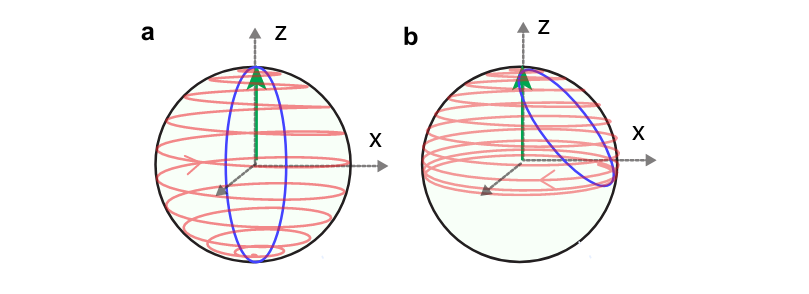
\includegraphics[width=\textwidth]{images/rabi_RWA.png}
    \caption{La linea rossa (blu) rappresenta l'evoluzione di un qubit guidato nel sistema del laboratorio (sistema rotante del drive). \textbf{a} con $\Delta=0$ e \textbf{b} per $\Delta \neq 0$. \url{https://arxiv.org/pdf/1904.09291.pdf}}
    \label{fig:my_label}
\end{figure}

\subsection{Controllo XY}
Consideriamo ora l'hamiltoniana per un qubit TRANSMON accoppiato tramite una capacità a una sorgente che porta un termine dipendente da $\sigma_y$ tale che:
\begin{equation*}
    \hat H= - \hbar \frac{\omega_q}{2}\hat \sigma_z + A(t) \hat \sigma_y
\end{equation*}
Passo al sistema di riferimento in rotazione con $\hat U = e^{-\frac{i}{\hbar}\omega_q t}$.
In questo sistema potrò applicare rotazioni sia rispetto all'asse x che rispetto all'asse y.
L'hamiltoniana si potrà scrivere come:
\begin{equation*}
    \hat H = U H_d U^\dagger = A(t) \left[ \cos \left( \omega_q t \right)\sigma_y -  \sin \left( \omega_q t \right)\sigma_x \right]
\end{equation*}
In questo caso scegliamo $A(t) = A v(t)$ ponendo attenzione non solo sull'ampiezza, ma anche sulla fase:
\begin{equation*}
    v(t) = s(t) \sin \left( \omega_d t + \phi \right)
\end{equation*}
Dove $s(t)$ è una funzione adimensionale che funge da \textit{envelope} e mi porta a poter scrivere l'ampiezza come $As(t)$, mentre la fase $\phi$ è scelta arbitrariamente.
Possiamo riscrivere $v(t)$ come:
\begin{equation*}
    v(t) = s(t) \left( \cos (\phi) \sin (\omega_d t) + \sin (\phi) \cos (\omega_d t) \right)
\end{equation*}
La notazione più in voga per questi termini (che riconosciamo essere le due quadrature del segnale RF) ci dice:
\begin{align*}
    I &= \cos \phi \qquad \text{chiamata per ragioni storiche: componente in fase} \\
    Q &= \sin \phi \qquad \text{chiamata per ragioni storiche: componente fuori fase} 
\end{align*}
E abbiamo le proprietà:
\begin{equation*}
    Q^2 + I^2 = 1 \qquad , \qquad \phi = \arctan\frac{Q}{I}
\end{equation*}
E riscriviamo la nostra hamiltoniana come:
\begin{equation*}
    \hat H = As(t) \left[  I \sin (\omega_d t) - Q \cos (\omega_d t)  \right]\times \left[ \cos (\omega_q t) \sigma_y - \sin (\omega_q t) \sigma_x \right]
\end{equation*}
Svolgendo il prodotto, usando un po' di trigonometria e applicando la RWA (rimuovo i termini dipendenti da $\omega_q + \omega_d$) arrivo a:
\begin{equation*}
    \hat H = \frac{1}{2}As(t) \left[ \left(-I \cos ( \Delta t) + Q \sin ( \Delta t) \right) \sigma_x + \left(I\sin ( \Delta t) - Q \cos ( \Delta t)  \right) \sigma_y \right] 
\end{equation*}
Che, espressa in forma matriciale, diventa:
\begin{equation*}
    \hat H = -\frac{A}{2}s(t) \begin{pmatrix} 0 & e^{i (\Delta t + \phi)} \\ e^{-i (\Delta t + \phi)} & 0 \end{pmatrix}
\end{equation*}